\chapter{Election Maps}

\section{Introduction}\
The ability to display geographically oriented data on maps is an 
indispensable tool for statisticians.
Election results are one example of such data, for votes are tallied according 
to political boundaries.
Well known to all of us is the map (Figure~\ref{fig:statemapredbluelarge})
that displays the results of the 2004 US presidential election
where each state is colored red for Republican or blue for Democrat according 
to whether Bush or Kerry received the most votes in the state. 
We explore alternative ways for displaying these 
election results that attempt to overcome some of the most
obvious drawbacks of this map--

\begin{figure}
\includegraphics{electionMaps/statemapredbluelarge.pdf}
%\epsfig{file=statemapredbluelarge}
\caption{ }
\label{fig:statemapredbluelarge}
\end{figure} 

\begin{itemize}
\item The map in Figure~\ref{fig:statemapredbluelarge} gives the false impression
that about 3/4 of the country voted Republican because
land area does not accurately represent population.
The red states cover far more geographic area than the blue ones, but
they have smaller populations than the blue states; in other words,
the blue states are small in area but large in terms of voters.
Across the United States, Bush received approximately 62 million votes (51\%) 
in the election,
Kerry received about 59 million (48\%) and Nader 400,000 (1\%), a far cry from 
the red-blue land area comparison. 

\item Further, in many states the election was quite close.
In Iowa Bush received 50\% of the vote compared to 49\% for 
Kerry; in Ohio the split was 51\% (Bush) to 49\%; and in Pennsylvania
it was 51\% Kerry for to  49\% for Bush. 
Where a state lands on the continuum from 0 to 100\% voting Republican 
is not apparent in the map.
The vote in Ohio's closely contested race looks no different than
the vote in North Dakota, where Bush's support was 63\%.
In terms of electoral college votes these distinctions make little
difference because the candidate who wins the popular vote takes all of
the electoral college votes for that state, but the additional information 
is helpful for a more in-depth assessment of the popular vote. 
\end{itemize}

In this chapter we will make election maps that attempt to address these
and other issues. Our first step is to recreate the 
map in Figure~\ref{fig:statemapredbluelarge}.
To do this we need to 
\begin{itemize}
\item acquire the data (vote counts for each state)
\item find and learn how to use map-making software 
\item analyze and map the data
\end{itemize}
Once acquainted with the data and software at hand,
our next step includes a more in-depth analysis that considers
the two issues raised about geographic area and color.
Then in a third round of map making, we go further in our analysis to address
other issues such as the granularity of the information presented 
and whether additional information that is geographically oriented may 
bring more insight to and further enrich our map.
In all of these phases, the three tasks of data acquisition,
learning about software, and data analysis, and the interplay
between these three tasks, are very important  in the process
of creating our map.
For example, data analysis may lead to new ideas for mapping
the data which require us to learn more about how the software
works, or it may lead to ideas about other data to collect
and include in the map.  Reciprocally, the task of
finding and cleaning data may give us ideas about how to analyze and
map it, or exploring the software may provide alternative ideas for
presentation and data organization.
This chapter highlights this process as we twice revisit our 
main goal of producing an election map, each time delving more
deeply into these three tasks as our maps change and evolve.


\section{Get out the votes}

Our first task in making a map like the one shown in 
Figure~\ref{fig:statemapredbluelarge}
is to get the official vote tallies for each state.
A search on \URL{www.google.com} with the keywords
``2004 official presidential election results" points us to
a Wikipedia site that has ``certified results" by state.
A little more snooping brings us 
to the Federal Election Commission website
and the official voting tallies for
each state can be found in a six-page pdf file 
at \URL{www.fec.gov/pubrec/fe2004/2004presgenresults.pdf}
(Figure~\ref{fig:officialElRes} contains a few snippets of it).
We see that over a dozen candidates ran for president from
parties that include the American Independent, Green,
Independent, Libertarian, and Peace and Freedom.

\begin{figure}
\includegraphics[height=2in,width=6in]{electionMaps/officialElRes1.pdf}
\includegraphics[height=2in,width=6in]{electionMaps/officialElRes2.pdf}
\includegraphics[height=2in,width=6in]{electionMaps/officialElRes3.pdf}
%\epsfig{file=officialElRes1,height=2in,width=6in}
%\epsfig{file=officialElRes2,height=1.5in,width=6in}
%\epsfig{file=officialElRes3,height=1.5in,width=6in}
\caption{ }
\label{fig:officialElRes}
\end{figure}
 
Other sites that appear high in Google's ranking include those
of news agencies, such as CNN, CBS, and USA Today.
The USA Today site 
\begin{verbatim}
http://www.usatoday.com/news/politicselections/vote2004/
  nationalelectionresultsbystate.aspx?oi=P&rti=G&cn=1&tf=l
\end{verbatim}
lists elections results from all
states on a single web page with each state in a separate table.
Whereas the CNN site presents each state separately, accessible
via a pull-down menu from\\
\URL{http://www.cnn.com/ELECTION/2004/pages/results/president/}.\\ 
On closer inspection of the voting results, we see that the CNN vote
counts exactly match those presented on the FEC site,
but the USA Today counts do not exactly. 
These discrepancies may be explained by the publication
dates of the data: the date on the document with the official government 
numbers is Feb 24, 2005, and those reported by USA Today have a date of 
Nov 11, 2004.  

Several options present themselves: although it is a bit more complicated to extract data
from a pdf formatted file, we could do this; we could also let Google
do the extraction for us (Google routinely provides HTML versions of
pdf files) and then extract the figures from the HTML;
we could pull the official numbers from the CNN site,
or the unofficial numbers from the USA Today site.
For the first map, we extract the data from the CNN site, and in a later
section we will use the USA today site because it offers an example of how to 
extract data remotely within R from web forms.

Refer to XML chapter for how to go about extracting the data.

Should  we add a function that creates a list(?) or
a  data-frame (?) or a CSV file from a html table?

PUT CODE HERE


\subsection{Map Software}
Our next task is to find software for making geographic maps.
Back on \URL{google.com} the search for 
``map software geographic open source" turns up many
sites related to open source Geographic Informations Systems.
GRASS GIS (Geographic Resources Analysis Support System) at 
\URL{grass.itc.it} looks promising.
The site \URL{opensourceGIS.org} provides scores of links to 
open source GIS-related software.
One that catches our eye is \URL{www.gstat.org}
which is described there as a computer program for geo-statistical
modeling, prediction, and simulation.
It is available as an R package and can read GRASS databases.
On closer inspection of the package on the Comprehensive R Archive
Network (CRAN) site at \URL{cran.us.r-project.org}, 
we find that the emphasis of the package is on
statistical modeling (kriging and variograms) not on mapping.
We also notice a GRASS R package that allows one to call R from
within GRASS.
Rather than pursue these angles, we look for other R packages 
that can make maps because our focus here is
on demonstrating how to find and learn about software not
on learning GIS systems (although that is a useful tool for
statisticians to have). A Google search for ``R geographic map"
turns up two packages, \RPackage{Rmap} and \RPackage{maps},
the later is on CRAN. A third search on Google, this time
for  ``R cran map" turns up a site 
\URL{http://sal.agecon.uiuc.edu/csiss/Rgeo/maps.html}
that describes the map-related R packages both on CRAN and not.  
These include,

\noindent 
\RPackage{mapdata} - Extra Map Databases;\\
\RPackage{mapproj} - Map Projections;\\
\RPackage{maps} - Draw Geographical Maps;\\
\RPackage{maptools} and \RPackage{shapelib} - Tools for reading and handling shape files;\\
\RPackage{rgdal} - provides bindings between R and GDAL for accessing
image and raster data.\\
\RPackage{RArcInfo} - provides an interface to read geographic information in
Arc/Info format.\\


It appears that \RPackage{maps} might work for us.
Packages on CRAN each have a web page where we can download the zipped package
source, view the index of the package contents, and read the reference
manual.
The documentation for the \RPackage{maps} package lists the functions in alpha order,
which is not all that helpful when trying to figure out how to start
to use a package.  We would prefer the central most important functions 
to be listed first in a general overview of the package with examples.
A search online does not uncover any vignettes or  tutorials on how to use the
\RPackage{maps} package, and skimming the contributed documentation on CRAN
we do not find any examples of maps.

Let's install the package and proceed from there  with our exploration of the
package's user philosophy.
To do this, we download and save the package source 
\verb+maps_2.0-27.tar.gz+.
The name of the package includes the version, 2.0-27.
[What does that mean?]...
Also we see on the web page that the package depends on
R version 1.7.0 or higher, since we are running version 2.0.1 
we should have no problems.
If we do have trouble, the maintainer of the package is
listed, and the reference manual contains his contact information.
Also, we can post questions to the R help mailing list 
at \URL{http://www.r-project.org/mail} or
check on the help mailing-list archive to see if our question has 
been answered already. 
(Currently there are about 500 messages referring to the 
\RPackage{maps} package on the archive).
Finally, this page also tell us that the software has a GPL2 license
[WHAT does that mean]...

Once we download the package, to install it we simply run 
R with additional run time arguments:
\begin{verbatim}
R CMD INSTALL maps_2.0-27.tar.gz
\end{verbatim}
[WHAT about environment variables....]
[ What about Mac vs windows vo linux]

Now to continue our research on how the package works, we look for a demo.
The command
\begin{verbatim} 
> demo(package = .packages(all.available = TRUE))
\end{verbatim}
indicates there are no demos for \RPackage{maps}.
Next, we turn to the R help facilities, we start the R help in our browser,
\begin{verbatim}
> help.start()
\end{verbatim}
and look up the \RPackage{maps} package. 
There we find a list of the functions that are documented. 
These  form a subset of the functions that are part of the package. 
The others are not documented because they are generally for internal
use by the package, not the user. 
To see the complete list of functions, 
we call \SFunction{objects} with the argument $3$, 
\begin{verbatim}
> objects(3)
 [1] "apply.polygon"        "area.map"             "area.polygon"        
 [4] "as.matrix.polygon"    "centroid.polygon"     "char.to.ascii"       
 [7] "closed.polygon"       "gp.smooth"            "identify.map"        
[10] "in.one.polygon"       "in.polygon"           "indicators.factor"   
[13] "insert"               "is.regexp"            "kernel.region.region"
[16] "kernel.region.x"      "kernel.smooth"        "makepoly"            
[19] "map"                  "map.axes"             "map.cities"          
[22] "map.old"              "map.poly"             "map.scale"           
[25] "map.text"             "map.where"            "map.wrap"            
[28] "mapgetg"              "mapgetl"              "mapname"             
[31] "mapthin"              "maptype"              "match.map"           
[34] "match.map.grep"       "match.map.slow"       "num.polygons"        
[37] "range.polygon"        "smooth.map"           "sub.polygon"         
[40] "subgroup"            
\end{verbatim}
The argument of $3$ tells R where in the search path for our session
to find \SPackage{maps},
\begin{verbatim}
> search()
 [1] ".GlobalEnv"        "package:mapproj"   "package:maps"     
 [4] "package:methods"   "package:stats"     "package:graphics" 
 [7] "package:grDevices" "package:utils"     "package:datasets" 
[10] "Autoloads"         "package:base"     
\end{verbatim}
We see that the package of interest is the third in line in the search path,

We have found that \SFunction{map} is the main entry
point in the package. To get a quick idea for the user-model for
the package, we run the examples provided by the documentation for
\SFunction{map},
\begin{verbatim}
> example(map)
\end{verbatim}
We discover that the simple command \verb+map("state")+ is a 
good starting point.
It provides a state map of the 48 contiguous states.
The example code for \SArg{state} fills the states with
colors.
\begin{verbatim}
map('state', fill = TRUE, col = palette() )
\end{verbatim}

Before making our election map, we need to understand better the map interface.
The documentation for the \Sfunction{map} function provides 
a simple form: 
\begin{verbatim}map(database, regions)
\end{verbatim} 
where the argument \SArg{database} is described as a
\begin{quote}
character string naming a geographical database, or a list of x, y, and names obtained
from a previous call to map. The string choices include a world map, three 
USA databases (usa, state, county), and more (see the package index). 
\end{quote}
The second argument, \SArg{regions} takes a character vector that names the polygons 
to draw. For example, the state of California is one such polygon in the 
state database.  According to the documentation, for those states 
composed of more than one polygon, 
the individual polygons have the name of the region, 
followed by a colon and a qualifier, as in michigan:north and michigan:south. 
The \SArg{exact} argument is boolean used to specify whether exact matching
(\STrue) or regular expressions are used in matching region names.

Given, the state map example in the documentation, it appears that the 
\SArg{fill} and \SArg{col} arguments are needed to color states red and blue. 
According to the documentation, the \SArg{col} argument takes a vector of colors. 
When the \SArg{Fill} argument is \STrue then 
``the colors are matched one-one with the polygons that get selected by the 
region argument (and are reused cyclically, if necessary)." 

To learn more about the databases that the function takes, we refer to
the documentation for \SVariable{state} describes it as a follows:
\begin{quote} 
The data file is merely an assignment to a character string which specifies 
the name of an environment variable which contains the base location of the 
binary files used by the map drawing functions. 
This environment variable (R\_MAP\_DATA\_DIR for the datasets in the maps package) 
is set at package load time if it does not already exist. 
\end{quote}

Overall, the documentation does not completely satisfy us and we turn to
the references listed there.
The paper, ``Maps in S", by the authors of the 
original code, Becker and Wilks, looks promising.
According to them,

\begin{quote}
The map function is an interface to geographical databases. 
%In developing its capabilities we have used data supplied by the US Census Bureau 
%(see References), which describes all county boundaries in the United States. 
%From this data we constructed three geographical data-bases with information
%on national, state and county boundaries in the USA. 
...
The information in each geographical database is organized into three files. 
The first file has descriptions of polylines. 
These are sequences of points on the earth's surface, which, when joined in order 
by line segments, form a part of the map, typically a political or natural boundary. 
The second file describes polygons in terms of polylines, 
that is, each polygon is given as a list of polyline numbers, 
indexing polylines from the polyline file, which, 
when traversed in the given order, form a closed area of the map. 
Finally, a third file gives names to each of the polygons in the second file. 
It is primarily through these names that the map data is accessed. 
Polygons are named with a convention that allows several polygons to be accessed with
one name, such as referring to the two parts of Michigan with the name ``Michigan.''
\end{quote}

To summarize the process just completed, to look for entry points
in unfamiliar software and to understand the philosophy behind
the use interface, we  

\begin{itemize}
\item search the web for vignettes and tutorials 
\item run demos and examples, such as with \SFunction{demo}
and \SFunction{example}
\item call up the help system, e.g. \SFunction{help.start}
\item read package documentation 
\item track down references in the documentation 
\item search the mailing list archive
\item look for other, undocumented entry points, e.g. \SFunction{objects}
\end{itemize}

Armed with this information about \RPackage{maps}, 
we turn our attention to reproducing the map in 
Figure~\ref{fig:statemapredbluelarge}.

\subsection{Analysis and map making}
The analysis of our data is straightforward in this phase:
we compare vote counts to determine the winner in each state.
For these purposes we can simply compare votes for Bush to votes for
Kerry and ignore the results from the other candidates.
The object \SVariable{stateColor} is a character vector of length 49
for the 48 contiguous states plus the District of Columbiacolumvbia.
The values are ``red" or ``blue" according to whether Bush or 
Kerry won the popular vote in the state. The names of the 
elements are the corresponding state names. 
\begin{verbatim}
> map("state", names(stateColor), col = stateColor, fill = TRUE)
\end{verbatim}
The resulting map is in Figure~\ref{fig:statemapwrong}. 
Something went wrong; New Jersey, New York, Pennsylvania, and 
Washington are red instead of blue.

\begin{figure}
\includegraphics[height=3in]{electionMaps/statemapwrong.pdf}
%\epsfig{file=statemapwrong,height=3in}
\caption{Notice that Pennsylvania, New Jersey, New York, and Washington are red.}
\label{fig:statemapwrong}
\end{figure} 

To trouble shoot the problem we:

\begin{itemize}
\item Check our input vector for correct matching of
state name and color: There does not appear to be a problem
with our input.

\item Try a few simple cases to see if we get what we expect:  
A plot of the region consisting of
Minnesota, Michigan and Texas with the colors red, blue and green,
in that order, yields a surprising result (see Figure~\ref{fig:michigantexas}).
Given our understanding so far, we expect Minnesota to be red, Michigan blue, 
and Texas green. Instead we see that Minnesota is green and Michigan has 
two colors. 
 
\begin{verbatim}
> map("state")
> map("state", c("minnesota","michigan","texas"),
      col = c("red","blue","green"), fill = TRUE, add = TRUE)
\end{verbatim}

\begin{figure}
\includegraphics[height=3in]{electionMaps/michigantexas.pdf}
%\epsfig{file=michigantexas,height=3in}
\caption{A call to the map function with the region Minnesota, Michigan and Texas
and the colors red, blue and green, produced a plot with Minnesota green not red,
Texas red not green, and Michigan two colors.}
\label{fig:michigantexas}
\end{figure} 

\item Save and examine the results from a call to the function:
\small{
\begin{verbatim}
> mapResult = map("state", plot = FALSE)
> class(mapResult)
[1] "map"
> names(mapResult)
[1] "x"     "y"     "range" "names"
> length(mapResult[[ "names" ]])
[1] 63
> mapResult[[ "names" ]][ 53:63 ]
 [1] "virginia:chesapeake"        "virginia:chincoteague"     
 [3] "virginia:main"              "washington:san juan island"
 [5] "washington:lopez island"    "washington:orcas island"   
 [7] "washington:whidbey island"  "washington:main"           
 [9] "west virginia"              "wisconsin"                 
[11] "wyoming"                   
\end{verbatim}
}
The output from a call to \SFunction{map} is an object of 
class map with four elements, \SVariable{x}, \SVariable{y},
\SVariable{range}, and \SVariable{names}.
There appear to be 63 named regions, each corresponding to a polygon,
and named according to the convention described in the previous section.
The name matching apparently does not work the way we expected.

\item Return to the documentation and read it more carefully: 
In the documentation for \SFunction{map} and \SVariable{state}
we do not see a mention of this issue, but we discover the 
function \SFunction{match.map}, which assigns an index to 
each map region and is ``useful for map coloring."

\small{
\begin{verbatim}
> colorIndex = match.map("state", names(stateColor))
> colorIndex
 [1]  1  2  3  4  5  6  7  8  9 10 11 12 13 14 15 16 17 18 19 20 20 20 21 21 22
[26] 23 24 25 26 27 28 29 30 31 31 31 31 32 32 32 33 34 35 36 37 38 39 40 41 42
[51] 43 44 45 45 45 46 46 46 46 46 47 48 49
\end{verbatim}
}
\end{itemize}

The example in match.map shows how to solve the problem.
\begin{verbatim}
map("state", names(stateColor), col = stateColor[colorIndex], fill = TRUE)
\end{verbatim}
We now have a map that is in agreement with Figure~\ref{fig:statemapredbluelarge}.


\section{One acre one vote}
In our example, the geographically oriented data the unit of interest is
typical population, not 
Election results pertain to people. 
Geographic information, where the people live 
Maps of election results aim to show who voted for Bush or Kerry and where they live. 
A difficulty that arises with adding population information to geographic maps pertains
to the uneven population density in the region. 
The colored maps shown here fill the state region with a color to indicate 
how the people of the voted, 
but the states with lower population densities are over-represented in these maps.

Cartograms reshape the map while maintaining geographic boundaries, 
so the area of the regions are proportional to the variable of interest, 
which is population in our case. 
Statisticians, cartographers, and physicists have considered the problem of 
constructing cartograms for the 2004 presidential election results. 
See for example, the cartograms of Venkatasubramanian (Figure~\ref{})
and Gastner, Shalizi, and Newman (Figure~\ref{}).
The later group uses the linear diffusion process of elementary physics to 
create a map where the geographic boundaries are distorted to represent population. 
That is, given a particular population density, they allow the population to 
flow away from high-density areas, stretching the boundaries of regions, in order
to equalized the density everywhere.


\begin{figure}
\includegraphics[height=3in]{electionMaps/venkatasubramanian.pdf}
\includegraphics[height=3in]{electionMaps/gastnerNewman.pdf}
%\epsfig{file=venkatasubramanian,height=3in}
%\epsfig{file=gastnerNewman,height=3in}
\caption{}
\caption{}
\label{fig:cartograms}
\end{figure}

\begin{figure}
\includegraphics{electionMaps/stateCirclesRB.pdf}
%\epsfig{file=stateCirclesRB}
\caption{}
\label{fig:stateCirclesRB}
\end{figure}

For a more simplistic approach that does not distort the geographic region,
but uses color in areas that are proportional to population, we superimpose symbols
of different sizes on the map at appropriate locations.
Figure~\ref{fig:stateCirclesRB} is an example. 
The area of the circles is proportional to the voters in the state, 
and the center of each circle is placed at the center of the corresponding state.
To add the circles to the states, we must find the state centers.
The \SPackage{maps} package documentation lists several 
internal functions related to polygons, which we can also see
with a call to \SFunction{objects}.
\begin{verbatim}
area.polygon(p) 
centroid.polygon(p) 
as.matrix.polygon(x) 
closed.polygon(p) 
in.one.polygon(p, x)
in.polygon(p, x) 
num.polygons(p)
range.polygon(..., na.rm = FALSE) 
sub.polygon(p, i) 
\end{verbatim}

These functions are not exported to the user.
That is, a call to help does not reveal any documentation on how to use 
these functions because it is expected that we will not need them.
However, the source code for \SFunction{centroid.polygon}
is well enough documented for us to figure  out that if we call 
it passing the \SArg{x},\SArg{y} coordinates of the 
polylines of the polygon of interest, then it returns the centroid
of that polygon.
To get the polylines, we store the results from a call to 
\SFunction{map} to plot the \SArg{state} database, which we know 
has vectors \SArg{x},\SArg{y} corresponding to the polylines
for the state polygons with the coordinates for each polygon
marked by \SNA.  We write the function \SFuntion{polys} to 
split up these vectors into a list of vectors, one for each
polygon. Then all we need to do is apply the \SFunction{centroid.polygon} 
function to each element of our list. Finally, we discard the extra polygons for 
those states made up of more than one polygon. 
\begin{verbatim}
mapR = map("state", plot=FALSE, fill= TRUE)
statePolys = polys(mapR[["x"]],mapR[["y"]])
stateCenters = sapply(statePolys, centroid.polygon)

#pick out index for one polygon from each state
onePoly = sort( c( (1:63)[- grep(":",mapR[["names"]])],
                          grep(":south",mapR[["names"]]),
                          grep(":main",mapR[["names"]]) ) )
stateCenters1 = stateCenters[ onePoly,]
\end{verbatim}

How do we decide on the size of the circles? 
We make the area proportional to the number of voters, 
which implies the radius is proportional to the square root of voters.
We further scale the total number of voters in the state by the 
maximum over all states so it fits the scale of the map.
\begin{verbatim}
# determine the radius of each circle
totalVote = bushVote + kerryVote
maxV = max(totalVote)
stateRad = 3*sqrt(totalVotes/maxV)

# determine the color of each circle
colorsRB = ifelse(bushVote > kerryVote, 
               rgb(1, 0, 0, 0.5), rgb(0, 0, 1, 0.5))

map("state")
symbols(stateCenters1[1,], stateCenters1[2,], circles = stateRad,
         add = TRUE, inches = FALSE, fg = colorsRB, bg = colorsRB)
\end{verbatim}

The circles give a much more accurate representation of the support
for Bush versus Kerry. They have been colored using transparency, which
allows us to see the overlapping states in the densely populated
northeastern part of the country.


\section{Winner take all}
Continuous data are often collapsed or transformed into categories or factors. We do this for many reasons: convention dictates it, data reduction makes the task manageable, or the categories are relevant to the analysis. But data reduction can yield a misleading or less-informative analysis. Take for example the map shown below, which appears on the USA Today website . Here, the percentage of votes for Bush in a county in the 2004 presidential election are converted to the categorical information as to whether Bush won or lost the vote in the county. A county is colored red for a Bush win and blue for a Bush loss (Kerry win). What information loss is there?

\begin{figure}
\includegraphics{electionMaps/stateTherms.pdf}
%\epsfig{file=stateTherms}
\caption{}
\label{fig:stateTherms}
\end{figure}

\begin{figure}
\includegraphics[height=3in]{electionMaps/bushPropHist.pdf}
%\epsfig{file=bushPropHist,height=3in}
\caption{}
\label{fig:statePropHist}
\end{figure}

\begin{figure}
\includegraphics{electionaps/stateSquareBrewerLegend.pdf}
%\epsfig{file=stateSquareBrewerLegend}
\caption{}
\label{fig:stateSquareBrewerLegend}
\end{figure}

\begin{figure}
\includegraphics{electionMaps/stateBrewerTrans.pdf}
%\epsfig{file=stateBrewerTrans}
\caption{}
\label{fig:stateBrewerTrans}
\end{figure}


However, with these two maps we can't tell if Bush won by a landslide, if the election was close, or if he lost by a landslide in the counties and states (respectively). That is, we have lost the information as to how close the election was in the county or state. Robert Vanderbei at Princeton University suggests using shades of purple to indicate the percentages of votes cast for Bush versus Kerry. His map appears below,

We get a much different impression of the voting patterns of Americans from this map. However, one drawback with the use of purple that has been pointed out at  http://homepage.mac.com/tcp/PurpleAmerica/

    Red shades tend to stand out more to the human eye than blue shades of the same saturation. As such a blended or ``purple" map of the US, based on the popular vote will tend to look a little more red than blue in its hue, given the bias of the human eye. 

See Brewer notes - we can get help outside of R

Purple maps in the press - problem is that they look red to the eye

Schema for color - depends on whether the data trying
to portray are sequential, diverging, or qualitative
Explain each of these and give some examples

How to specify colors in R that are more than Red and blue?
RGB is one way.

brewer.pal

How many variations in color do we use?
How do we determine the intervals? We can use percentiles,
percentages, square root, log....

Now the circle can be reduced to one 


\section{Granularity}
Level of the data - we can't know how an individual
votes, only the tally of results from a polling place,
or precinct.

County level data

Granularity of data --

For precinct level results we  
need to visit the individual State Records offices,
overseen by the Secretary of State.
The urls for these can be found at the 

\URL{http://www.fec.gov/pubrec/staterec.htm}

States are not obligated to store their data in same format.
Take Alabama and Wyoming for example. 

Alabama
Office of the secretary of State for the State of Alabama.

\URL{http://www.sos.state.al.us/election/2004/index.cfm}


to obtain an Excel files

Wyoming on the other had offers pdf files, one per precinct,
available at 

http://soswy.state.wy.us/election/2004/results/04-g-pp.htm

Precinct level is hard to come by. 
State level is easier. We can extract the official results from
the pdf file (HOW)
or use the election results posted on the web by the 
news agencies, such as USA Today and CNN. 
\begin{verbatim}
http://www.usatoday.com/news/politicselections/vote2004/
      nationalelectionresultsbystate.aspx?oi=P&rti=G&cn=1&tf=l
\end{verbatim}

% Change the sp=
%http://www.usatoday.com/news/politicselections/vote2004/PresidentialByCounty.aspx?oi=P&rti=G&sp=NJ&tf=l

This is how we can use XPath to get the data.

By looking at the HTML for NJ  (and MA), we can see that the 
first row of the table of interest start with 
\begin{verbatim}
<td class="notch_white" width="153"><b>Atlantic</b></td>
\end{verbatim}
It is the notch_white that identifies this table.
One has to make certain of this.
But if we could find that node and then go up
the tree from that to find its parent -- the row (tr) --
and then its parent -- the table, 
we could sweep over all the children and extract the
data.
So, if we use the following code
\begin{verbatim}
z = htmlTreeParse("http://www.usatoday.com/news/politicselections/vote2004/PresidentialByCounty.aspx?oi=P&rti=G&sp=NJ&tf=l", useInternal = TRUE)
v = getNodeSet(z, "//td[@class='notch_white']")
tb =xmlParent(xmlParent(v[[1]]))
\end{verbatim}
Alternatively, we could find all td elements with
a class of notch_white or notch_light and a width.
\begin{verbatim}
v = getNodeSet(z, "//td[@width and @class='notch_light' or @class='notch_white']")
\end{verbatim}
(We need the width or we would pick up the note at the bottom of
the table of ``Vote returns will appear shortly...''.
But we could identify this as not having multiple td elements.)
This  gives all the cells of the table, not just the first element
of each row.  It also gives back the one without the width.
We can identify this as the ``last'' one or alternatively as the one
with more than one child
\begin{verbatim}
table(sapply(v, xmlSize))
v = v[sapply(v, xmlSize) == 1]
\end{verbatim}
Then, we can fetch the values for each cell with
\begin{verbatim}
vals = matrix(sapply(v, xmlValue), , 6, byrow = TRUE)
vals = as.data.frame(vals)
vals[-1] = sapply(vals[-1], function(x) as.integer(gsub(",", "", as.character(x))))
\end{verbatim}
Note that we have to handle the commas in the numbers
and it is easy to just remove them.

So we can put all of this in a function
\begin{verbatim}
getStateVotes =
function(state) {
  uri =paste("http://www.usatoday.com/news/politicselections/vote2004/PresidentialByCounty.aspx?oi=P&rti=G&sp=",state, "&tf=l", sep = "")
  z = htmlTreeParse(uri, useInternal = TRUE)
  v = getNodeSet(z, "//td[@width and @class='notch_light' or @class='notch_white']")
  v = v[sapply(v, xmlSize) == 1]
  vals = matrix(sapply(v, xmlValue), , 6, byrow = TRUE)
  vals = as.data.frame(vals)
  vals[-1] = sapply(vals[-1], function(x) as.integer(gsub(",", "", as.character(x))))
  vals
}
\end{verbatim}

To get all the state abbreviations, we looked up ``state
abbreviations'' on the web and cut and pasted the results into
We should do this properly.
\begin{verbatim}
abbrevs = readLines("~/Classes/StatComputing/Book/electionMaps/stateAbbrevs")
abbrevs = abbrevs[nchar(abbrevs) == 2]
\end{verbatim}
This gives 59 values, yet we expected only 51 (including the
district of Columbia (DC)). We also get Western Samoa, etc.
So we either want to remove these or make the function
robust to handling errors in retrieving the URI.
And in fact it is.
\begin{verbatim}
stateVotes = lapply(abbrevs, getStateVotes)
names(stateVotes) = abbrevs
\end{verbatim}


Where do we get county centers?  -- learn more about the software

Why doesn't our circle show up?
do we need mapproject?

Use the locator function to see what's going on.
Place axes on the map so that we can see if we have the right units
We find that X and Y are reversed
We also find that X and Y are on the wrong scale

problem with jitter

problem with cex

\subsection{reconciling the differences between various sources}

Missing counties

Counties with different names

Parish, Bourough, Townships and Counties


\section{Additional data}

\subsection{Census data}
How to get it

Antoehr data source to reconcile

How to portray it

\subsection{Adding Markers to the Map}    

cities\\
titles\\
legends\\
map markers do not all work the same way as the plot function



=========================================

[A CHAPTER on GIS?  -- or include it as an example of Intersystem interfaces? ]

%Notice that the data are a bit more complicated because there are
%more candidates running than Bush and Kerry
%In Alaska Nader, Peroutka (American Independent), Badnarik (Libertarian), 
%and Cobb (Green)
%In Arizona only Bush, Kerry and Badnarik
%In California Badnarik, Cobb, Peltier (Peace and Freedom), and Peroutka 

%We examine a few other packages, and read the 
%accompanying documentation.

%Although we are not interested in the map of china and new zealand
%found in mapdata package we may be interested in the map,world

%mapproj converts latitude and longitude into projected coordinates.
%map.grid draws a grind on an existing map
%maproject converts latitude and longitude into projected coordinateso

